% xetex compatible variant that support TTF fonts according to company rules
\documentclass[ignorenonframetext, professionalfonts, hyperref={unicode}]{beamer}

\usetheme{Epam}

\usepackage{fontspec}
\setsansfont{SourceSansPro-Regular}
%\setbeamerfont{frametitle}{family=\fontspec{Oswald}}
\setbeamerfont{frametitle}{family=\fontspec{Oswald}}
\setbeamerfont{block title}{family=\fontspec{Oswald}}

%\setmainfont{Times New Roman}
\defaultfontfeatures{Mapping=tex-text}
\defaultfontfeatures{Ligatures=TeX}

%\setsansfont{Arial}
%\setromanfont{Trebuchet MS}

\usepackage{cmap}
\usepackage{graphicx}

\usepackage{textcomp}

\usepackage{beamerthemesplit}

\usepackage{ulem}

\usepackage{verbatim}
\usepackage{import}

\usepackage{listings}
\lstloadlanguages{bash}

\lstset{escapechar=`,
	captionpos=b,
	extendedchars=false,
	language=sh,
%	frame=single,
	tabsize=2, 
	columns=fullflexible, 
%	basicstyle=\scriptsize,
	keywordstyle=\color{blue}, 
	commentstyle=\itshape\color{brown},
%	identifierstyle=\ttfamily, 
	stringstyle=\mdseries\color{green}, 
	showstringspaces=false, 
	numbers=left, 
	numberstyle=\footnotesize, 
	breaklines=true, 
	inputencoding=utf8,
	keepspaces=true,
	morekeywords={u\_short, u\_char, u\_long, in\_addr}
	}

\definecolor{darkgreen}{cmyk}{0.7, 0, 1, 0.5}

\lstdefinelanguage{diff}
{
    morekeywords={+, -},
    sensitive=false,
    morecomment=[l]{//},
    morecomment=[s]{/*}{*/},
    morecomment=[l][\color{darkgreen}]{+},
    morecomment=[l][\color{red}]{-},
    morestring=[b]",
}

\author[Epam]{{\bf Epam}\\Low Level Programming Department}

%\institution[EPAM]{EPAM}
%\logo{\includegraphics[width=1cm]{logo.png}}

\graphicspath{{../../slides/cmdline/clipart/}{../../slides/bash/clipart/}}

\bibliographystyle{unsrt}
\setbeamertemplate{bibliography item}{\insertbiblabel}

\AtBeginSection[]{%
  \begin{frame}<beamer>
    \frametitle{}
    \tableofcontents[
        sectionstyle=show/shaded, hideallsubsections ]
  \end{frame}
  \addtocounter{framenumber}{-1}% If you don't want them to affect the slide number
}

% \regex for regular expressions
\newcommand{\regex}[1]{ %
\expandafter{$\ulcorner{\color{blue}\texttt{#1}}\lrcorner$} %
}



\title{Введение в GNU/Linux}

%%%%%%%%%%%%%%%%%%%%%%%%%%%%%%%%%%%%%%%%%%%%%%%%%
%%%%%%%%%% Begin Document  %%%%%%%%%%%%%%%%%%%%%%
%%%%%%%%%%%%%%%%%%%%%%%%%%%%%%%%%%%%%%%%%%%%%%%%%

\begin{document}

\begin{frame}
	\frametitle{Monitoring.}
	\titlepage
	\vspace{-0.5cm}
	\begin{center}
	%\frontpagelogo
	\end{center}
\end{frame}


\begin{frame}
	\tableofcontents
	[hideallsubsections]
\end{frame}

%%%%%%%%%%%%%%%%%%%%%%%%%%%%%%%%%%%%%%%%%   
%%%%%%%%%% Content starts here %%%%%%%%%%
%%%%%%%%%%%%%%%%%%%%%%%%%%%%%%%%%%%%%%%%%

\section{Zabbix. Definition and terms.}
% features
\mode<all>{\begin{frame}[fragile]
    \frametitle{Задачи системы мониторинга}
        \begin{itemize}
            \item Сбор данных
            \item Анализ данных
            \item Отправка оповещений
            \item Хранилище данных истории
        \end{itemize}
\end{frame}}
\mode<all>{\begin{frame}[fragile]
    \frametitle{Zabbix дополнительно предоставляет}
        \begin{itemize}
            \item Сетевое обнаружение
            \item Построение графиков в режиме реального времени
            \item Возможности Веб мониторинга
        \end{itemize}
\end{frame}}
% terms
\mode<all>{\begin{frame}[fragile]
    \frametitle{Определения}
        \begin{itemize}
            \item \alert{Узел сети (Host)} \\
            Устройство в сети от которого можно получить данные \\
            Пример: Windows server, Switch, printer …
            \item \alert{Группа узлов сети (Hosts group)} \\
            Объединение узлов сети по какому-либо признаку \\
            Пример: Linux servers, Printers, Storage servers …
            \item \alert{Элемент данных (Item)} \\
            Данные полученные от устройства \\
            Пример: CPU Load, Free Memory, CPU Temp
            \item \alert{Триггер (Trigger)} \\
            Логическое выражение реагирующее на элемент данных \\
            Пример: CPU Temp > 100
        \end{itemize}
\end{frame}


}
\mode<all>{\begin{frame}[fragile]
    \frametitle{Определения}
        \begin{itemize}
            \item \alert{Событие (Event)}  \\
    Одиночное возникновение происшествия \\
    Пример: срабатывание триггера, регистрация агента
            \item \alert{Действие (Action)} \\
    Действие состоит из операций реагирования на событие \\
    Пример: отправка сообщения, запуск команды
            \item \alert{Шаблон (Template)} \\
    Набор сущностей (данные, триггеры …)
        \end{itemize}
\end{frame}}
\mode<all>{\begin{frame}[fragile]
    \frametitle{Задачи системы мониторинга}
        \begin{itemize}
            \item \alert{Оповещение} \\
Информационное сообщение отправленное пользователю
            \item \alert{Способ оповещения} \\
Канал связи, способ отправки оповещения \\
Пример: email, slack, telegramm, sms
            \item \alert{Удаленная команда} \\
Команда которую можно выполнить на удаленном узле
        \end{itemize}
\end{frame}}
\section{Architecture.}
\mode<all>{\begin{frame}[fragile]
    \frametitle{Архитектура}
    \center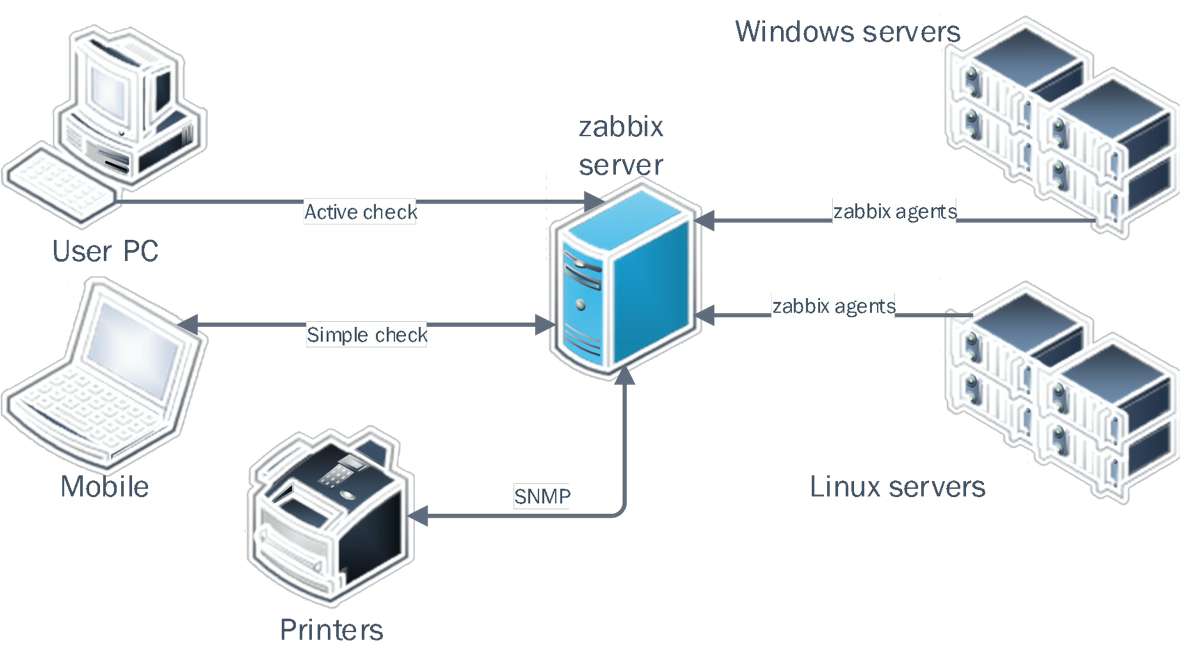
\includegraphics[width=11cm]{zabbix_arch}
\end{frame}}
\section{Installation.}
\mode<all>{\begin{frame}[fragile]
    \frametitle{Установка}
        \begin{itemize}
            \item Our goal:  \\
from the distribution packages
            \item Do it yourself: \\
Download the latest source archive and compile it yourself
            \item Modern methods: \\
Install it from the containers \\
Download the virtual appliance
        \end{itemize}
\end{frame}}
\section{Web Interface.}
\mode<all>{\begin{frame}[fragile]
    \frametitle{Изучаем интерфейс}
        \begin{itemize}
            \item добавить хост
            \item добавить метрики для мониторинга
            \item графики
            \item мониторинг веб
        \end{itemize}
\end{frame}}

\end{document}
